\pagestyle{empty} % Limpa o cabeçalho e o rodapé
\onehalfspacing % Espaçamento entre-linhas de 1,5
% \hyphenpenalty=10000 % To prevent hyphenation
\pretolerance=10000 % To avoid overflow lines
%\selectlanguage{english}
\selectlanguage{brazilian}
%\pagenumbering{arabic} % Uncomment this line if you want renumber pages for each chapter
\setcounter{ex}{0}
\renewcommand{\chaptername}{Tutorial}
\chapter{Manipulação de texto}\label{tut2}
\rhead{\tiny Instituto de Biociências --USP: BIZ0433 - Inferência Filogenética: Filosofia, Método e Aplicações}
\cfoot{\tiny \cc \ccby \ccsa \href{http://creativecommons.org/licenses/by-sa/4.0/}{Creative Commons Attribution-ShareAlike 4.0 International License}}
%\vspace{5pt}
{\large \sc BIZ0433 - Inferência Filogenética: Filosofia, Método e Aplicações.}\par
%\vspace{10pt}
\par
\minitoc % for table of contents within the chapter
\newpage
\section*{}\addcontentsline{toc}{section}{Objetivo}
\onehalfspacing
\vspace*{5pt}
\begin{center}
\emph{\begin{large}Objetivo\end{large}}\label{tut2:Objetivo}
\vspace{2pt}
\end{center}
%% TEXTO DO RESUMO
O objetivo deste tutorial é apresentar algumas ferramentas disponíveis em LINUX para visualizar e manipular arquivos textos. Aprender o básico sobre essas ferramentas é fundamental, pois todos os programas ou aplicativos que iremos utilizar durante o curso requerem dados de entrada e imprimem informações em arquivos textos. Este tutorial não explora de forma exaustiva todos os conceitos apresentados relacionados às ferramentas de manipulação de texto disponíveis. No entanto, introduz termos e conceitos, bem como comandos e aplicativos, que certamente lhes darão bases para executar muitas tarefas apresentadas ao longo do curso. Considerem, no entanto, que estas ferramentas poderão ser melhor estudadas fora da sala de aula à medida em que encontre necessidades especiais para executar determinadas operações. Os arquivos associados a este tutorial estão disponíveis no \href{https://github.com/fplmarques/cladistica/tree/main/tutorials/}{GitHub}. Você baixar todos os tutoriais com o seguinte comando:

\begin{center}
\small \texttt{svn checkout https://github.com/fplmarques/cladistica/trunk/tutorials/}\\
\end{center}

\newpage
\pagestyle{fancy} % Inclui o cabeçalho definido no meta.tex
%\pagenumbering{arabic} % Números das páginas em arábicos
\begin{refsection}
\renewcommand*{\finalnamedelim}{\addspace\&\space}% Usar '&' ao invés de 'e'.

%%%%%%%%%%%%%%%%%%%%%%%%%%%% HERE TEXT STARTS %%%%%%%%%%%%%%%%%%%%%%%%%%%% 
\section{Arquivos textos}\label{tut2:text}
	Uma das grandes vantagens dos sistemas Unix/Linux é que a grande maioria dos arquivos que gere e sustentam o sistema, bem como aqueles manipulados por aplicativos, são arquivos texto. Durante o curso, você verá que todos os arquivos de entrada (\textit{i.e.}, \textit{input files}) e saída (\textit{i.e.}, \textit{output files}), são arquivos aos quais você terá acesso direto via editores de texto ou que vocês serão capazes de imprimí-los diretamente no terminal para visualização. Adicionalmente, você notará que a manipulação (edição) de textos é muito comum. Isso porque arquivos de saída de determinados programas, ou parte deles, podem ser utilizados como arquivos de entrada para outros programas em análises subsequentes.\\

	Há uma lista de editores de texto disponíveis para todos os sistemas, mas o que queremos usar são aqueles que não inserem caracteres ocultos em seu arquivo (\textit{e.g.}, \textit{Word} da MicroSoft Windows). Dentre eles podemos citar \textit{Notepad} para sistemas Windows, \textit{TextWrangler} para MAC, e \texttt{vim}, \texttt{elvis}, \texttt{emacs}, \texttt{nedit}, \texttt{nano}, \texttt{kedit}, \texttt{gedit}, entre muitos outros para sistemas LINUX/UNIX. Para Linux, se o sistema no qual você está operando disponibiliza interfaces gráficas e seu ambiente de \textit{Desktop} é GNOME - como é o caso da imagem disponibilizada no curso - o \texttt{gedit} é um editor de texto muito versátil. Dentre aqueles que não requerem interface gráfica e, desta forma, são apropriados para uso em terminais, nós iremos adotar \texttt{nano}. Para aqueles que estiverem muito interessados em usar editores dessa natureza, considerem estudar o \texttt{emacs}, é inacreditável o que você pode fazer com ele! Ao explorar esses 
editores, considerem que o conforto e poder desses aplicativos são inversamente proporcionais \parencite [] [] {Wunchiers_2004,}!\\

\subsection{Editores de textos}\label{tut2:text:editors}

\subsubsection{GEdit}\label{tut2:text:editors:gedit}

Para abrir o \texttt{gedit} basta procurar o aplicativo no Painel Inicial do Ubuntu (veja Figura \ref{tut2:fig:gedit}) e digitar a palavra \texttt{gedit} ou verifique se ele já se encontra na barra lateral de aplicativos do seu sistema. Abra o \texttt{gedit} e com ele abra o arquivo \texttt{10\_tax\_all\_1000\_trees.tre} que está no diretório \texttt{tutorial\_02}. Veja as opções do programa na barra de menu e explore um pouco o que ele pode fazer. Note que ele não difere muito do que você está acostumado a fazer com o seu editor de texto (\textit{e.g.}, \textit{Word} da MicroSoft Windows). Este editor é intuitivo e eu acredito que não seja necessário explicar como ele funciona exceto pelo fato de que você pode abrí-lo diretamente via terminal com o comando:\\

\shellcmd{gedit \&}\\

\textcolor{red}{\textbf{Observação:}} O símbolo ``\texttt{\&}'' apenas faz com que o terminal rode o \texttt{gedit} no \textit{backgroud}. Se o ``\texttt{\&}'' é omitido, seu terminal fica vinculado à execução do \texttt{gedit} até que você feche o programa.\\

%%%%%%%%%%%%%%%%%%%%%%%%%%% FIGURA DO GEDIT %%%%%%%%%%%%%%%%%%%%%%%%%%%
%  \vspace{-1em}
  \begin{figure}[H]
    %\ffigbox[\FBwidth]
       \centering
      {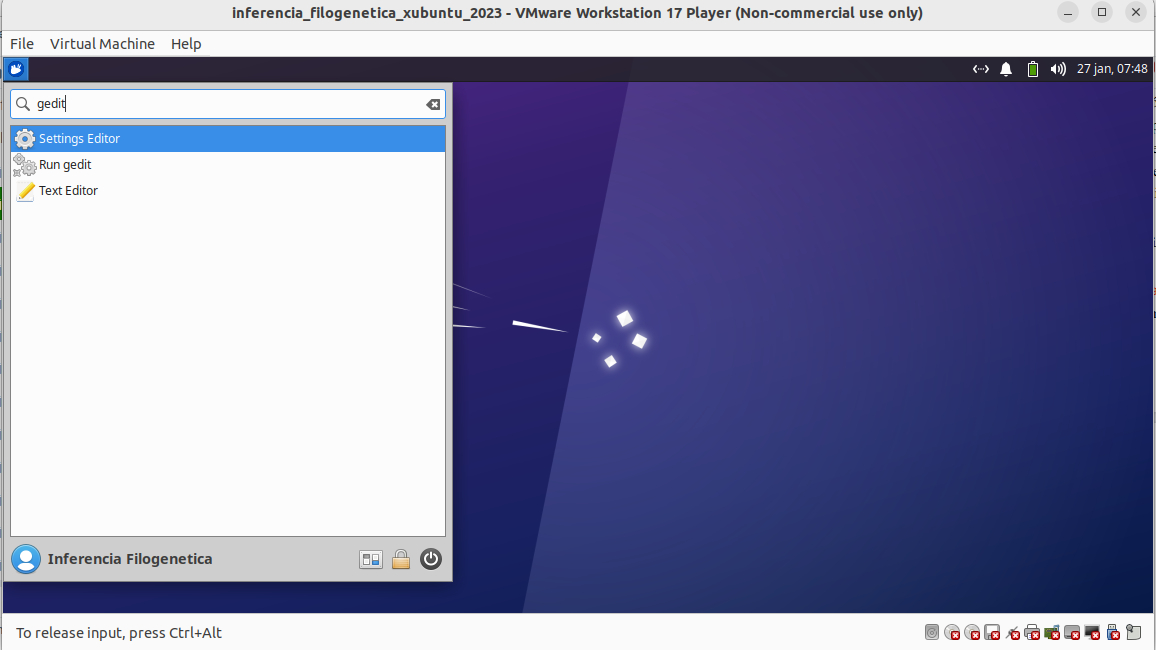
\includegraphics[scale=0.35]{figures/tut2/gedit.jpg}}
      {\caption[\textit{Abrindo \texttt{gedit} }]{Abrindo \texttt{gedit} na imagem de Xubuntu via Painel inicial. Observe que a barra lateral de seu sistema lhe permite acesso direto ao gedit.}\label{tut2:fig:gedit}}
  \end{figure}

%%%%%%%%%%%%%%%%%%%%%%%%%%% FIM DA FIGURA DO GEDIT %%%%%%%%%%%%%%%%%%%%%%%%%%%

\subsubsection{Nano}\label{tut2:text:editors:nano}

\texttt{Nano} é um editor que deve ser executado a partir de um terminal, e se concentra em simplicidade. \texttt{Nano} é um clone do antigo editor de texto \texttt{Pico}, o editor para o cliente de e-mail \texttt{Pine}, que foi muito popular lá pelos anos 90, em UNIX e sistemas do tipo LINUX. \texttt{Nano} foi criado em 1999 com o nome de \texttt{``TIP''} (uma sigla, um acrônimo recursivo que significa ``\texttt{TIP Isn't Pine}'', por Chris Allagretta. Allagretta decidiu criar este clone do \texttt{Pico} porque o programa não foi liberado sob a GPL. O nome foi mudado oficialmente em 10 de janeiro de 2000 para diminuir a confusão entre o novo editor e o comando ``\texttt{tip}'' (o comando ``\texttt{tip}'' é comum em Sun Solaris, uma distribuição de UNIX).\\
\texttt{Nano} usa combinações muito simples de teclas para trabalhar com arquivos. Um arquivo é aberto ou iniciado com o comando: \\

\shellcmd{nano <arquivo>}\\

Onde \texttt{<arquivo>} é o nome do arquivo que você deseja abrir.\\
Se você executa em um terminal o comando:\\

\shellcmd{nano teste.txt}\\


\texttt{Nano} irá abrir um arquivo vazio se \texttt{teste.txt} não existir no seu diretório de trabalho. No entanto, se você abrir o mesmo arquivo que abriu anteriormente utilizando \texttt{nano}, o arquivo \texttt{10\_tax\_all\_1000\_trees.tre} que está no diretório \texttt{tutorial\_02}, você deverá observar o terminal ilustrado na Figura \ref{tut2:fig:nano}.\\

%%%%%%%%%%%%%%%%%%%%%%%%%%% FIGURA DO NANO %%%%%%%%%%%%%%%%%%%%%%%%%%%
%  \vspace{-1em}
  \begin{figure}[H]
    %\ffigbox[\FBwidth]
       \centering
      {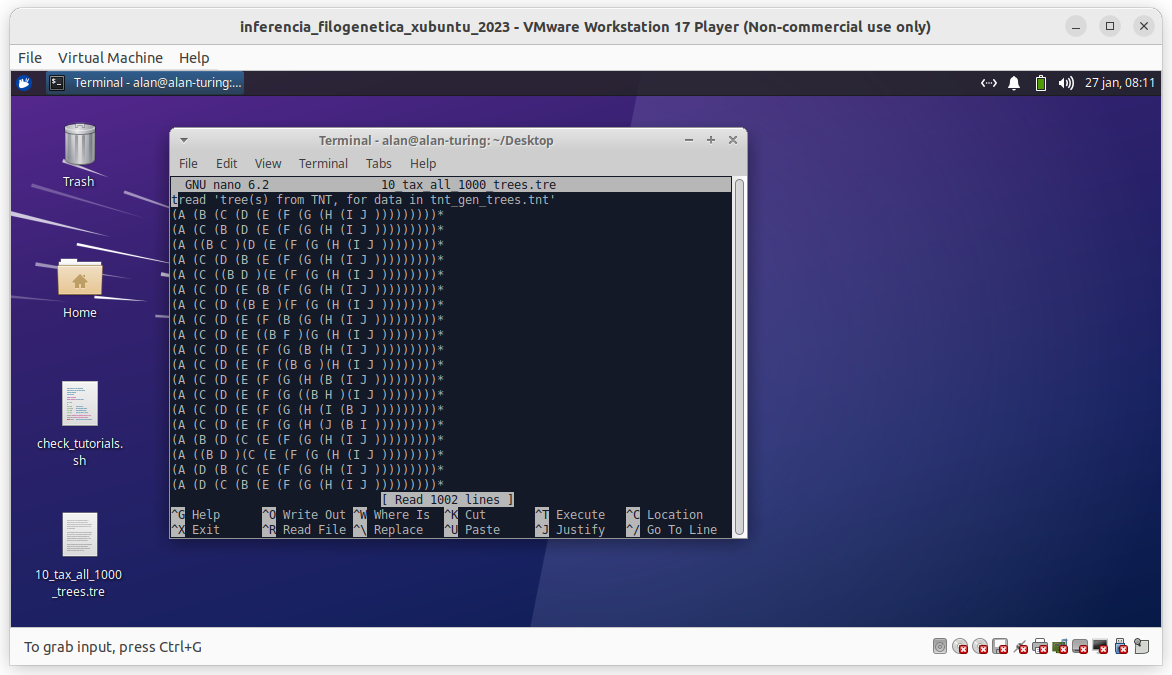
\includegraphics[scale=0.35]{figures/tut2/nano.jpg}}
      {\caption[\textit{Abrindo \texttt{nano} }]{Abrindo \texttt{nano} na imagem do Xubuntu via terminal.}\label{tut2:fig:nano}}
  \end{figure}

%%%%%%%%%%%%%%%%%%%%%%%%%%% FIM DA FIGURA DO NANO %%%%%%%%%%%%%%%%%%%%%%%%%%%

Quando o arquivo estiver aberto no \texttt{Nano}, você verá uma pequena lista de sintaxe de comando na parte inferior da janela do terminal (marcado em vermelho na Figura \ref{tut2:fig:nano}). Todas as combinações de teclas para \texttt{Nano} começam com a tecla \texttt{Ctrl}, o \texttt{Ctrl} convencionalmente é representado pelo símbolo ``\texttt{\^{}}''. Para executar um comando você deve manter a tecla \texttt{Ctrl} pressionada e clicar na segunda tecla para executar a ação. As combinações mais comuns para \texttt{Nano} são:\\

\noindent\textbf{\texttt{Ctrl-x}} - Sai do editor. Se você estiver no meio da edição de um arquivo, o processo de saída irá perguntar se você quer salvar seu trabalho.\\
\textbf{\texttt{Ctrl-R}} - Ler um arquivo em seu arquivo de trabalho atual. Isso permite que você adicione o texto de outro arquivo enquanto trabalha dentro de um novo arquivo.\\
\textbf{\texttt{Ctrl-c}} - Mostra a posição atual do cursor.\\
\textbf{\texttt{Ctrl-k}} - ``recorta'' o texto.\\
\textbf{\texttt{Ctrl-U}} - ``cola'' o texto.\\
\textbf{\texttt{Ctrl S}} - Salva o arquivo e continua trabalhando.\\
\textbf{\texttt{Ctrl-T}} - verifica a ortografia do seu texto.\\
\textbf{\texttt{Ctrl-w}} - faz uma busca no texto.\\
\textbf{\texttt{Ctrl-a}} - leva o cursor para o início da linha.\\
\textbf{\texttt{Ctrl-e}} - leva o cursor para o fim da linha.\\
\textbf{\texttt{Ctrl-g}} - mostra a ajuda do \texttt{Nano}.\\

Existem muitos outros comandos disponíveis em \texttt{Nano}. Para ver a lista de comandos, use o comando \textbf{\texttt{Ctrl-g}}.\\

\stepcounter{ex}
\begin{blackBlock}{\textbf{Exercício 2.\arabic{ex}}}\label{tut2:ex:2.\arabic{ex}}

Você deverá criar um arquivo chamado \texttt{matrix.txt} utilizando \texttt{Nano} com o seguinte conteúdo:\\

\texttt{p04 0000000}\\
\texttt{p02 1110000}\\
\texttt{p05 1110000}\\
\texttt{p06 1101000}\\
\texttt{p03 1101000}\\
\texttt{p01 1000100}\\
\texttt{p08 1000110}\\
\texttt{p10 1000111}\\
\texttt{p09 1000111}\\

\end{blackBlock}

\subsubsection{Outras formas de visualização de texto}\label{tut2:text:editors:texttools}

Há outras formas de visualizar e/ou obter informações rápidas de arquivos texto. Abaixo iremos explorar algumas delas:\\
\paragraph{Comando \texttt{cat:}}\label{tut2:text:editors:texttools:cat}
O comando \texttt{cat} foi introduzido a vocês no Tutorial \ref{tut1} (item \ref{tut1:text_mode:commands:cat}). Na ocasião, aprenderam que este comando permite a impressão do conteúdo de arquivos texto no terminal, bem como seu uso para concatenar arquivos textos utilizando os caracteres de direcionamento (\textit{i.e.}, ``\texttt{>}'' e ``\texttt{>>}''; veja item \ref{tut1:pipered} do Tutorial \ref{tut1}). No entanto, o comando \texttt{cat} pode também ser utilizado para criar arquivos de forma bem mais rudimentar do que o \texttt{nano}. Um exemplo é dado no próximo exercício.\\

\stepcounter{ex}
\begin{blackBlock}{\textbf{Exercício 2.\arabic{ex}}}\label{tut2:ex:2.\arabic{ex}}

Abra um terminal e digite:\\
\shellcmd{cat > tnt\_head.txt}\\

Você deverá obter uma linha vazia no terminal. Digite:\\
\texttt{``xread''} (sem as aspas)\\
Pressione \textsc{enter}.\\
Agora digite:\\
\texttt{``7 10''} (novamente sem as aspas)\\
Pressione \textsc{enter}.\\
Finalmente pressione  \texttt{Ctrl-D}\\

Examine o conteúdo de \texttt{tnt\_head.txt}:\\
\shellcmd{cat tnt\_head.txt}\\

Você deverá ter obtido um arquivo com o seguinte conteúdo:\\
\texttt{xread}\\
\texttt{7 10}\\
\end{blackBlock}

Muito bem! Você irá usar esse arquivo em breve, portanto deixe-o no diretório \texttt{tutorial\_02}.\\

\paragraph{Comando \texttt{sort:}}\label{tut2:text:editors:texttools:sort}
O \texttt{sort} é um programa interno de Linux que organiza as linhas de um arquivo texto ou da entrada padrão. A organização é feita por linhas e as linhas são divididas em campos que é a ordem em que as palavras aparecem na linha separadas por um delimitador (normalmente um espaço). Organizar aquivos pode facilitar muito a leitura, principalmente de tabelas e, em alguns casos ou seu arquivo é muito grande para ser organizado por programas como Excel ou você não terá acesso à interfaces gráficas. Portanto, o \texttt{sort} pode ser uma ferramenta muito poderosa para organizar informação.\\

\textit{Sintaxe:}\\
 \shellcmd{sort -opção1 -opção2 --opção3 argumento}

O \texttt{argumento} é, via de regra, o arquivo que contém as informações que você quer organizar. Há diversas opções para esse programa (veja \texttt{\$ man sort}, para maiores detalhes); no entanto, iremos apresentar algumas poucas que podem ser úteis utilizando alguns exemplos.\\

Veja uma utilidade simples deste programa. O arquivo \texttt{sort\_example\_1.tre} contém uma série de topologias compiladas pelo POY \parencite[][]{VaronETAL_2010, VaronETAL_2014} -- um programa desenvolvido para análises de homologia dinâmica, que veremos no Tutorial \ref{tut9}. Para saber o número de topologias contidas neste arquivo basta usar o comando \texttt{wc} com a opção \texttt{-l} (veja Tutorial \ref{tut1}, seção \ref{tut1:text_mode:commands:wc}). O programa \texttt{sort} tem o termo ``\texttt{-u}'' como uma de suas opções, nela são consideradas apenas as linhas que são únicas, ou seja, diferentes. Desta forma, a linha de comando:\\

\texttt{\$ sort -u sort\_example\_1.tre}\\

retorna apenas as topologias únicas contidas neste arquivo. \\

\stepcounter{ex}
\begin{blackBlock}{\textbf{Exercicio 2.\arabic{ex}}}\label{tut2:ex:2.3}

Quantas topologias únicas existem neste arquivo?.

\end{blackBlock}

\begin{center}
\line(1,0){400}\\
\end{center}

\vspace{30pt}


Veremos outras utilidades do \texttt{sort}. Verifique o conteúdo do arquivo \texttt{random\_taxon\_table.tsv} no diretório \texttt{tutorial\_02} utilizando o comando \texttt{cat}. A extenção ``\texttt{.tsv}'' (\textit{\textbf{T}ab \textbf{S}eparated \textbf{V}alues}) é utilizada para arquivos em que os valores ou conjunto de textos estão separados por \texttt{TAB}. Você consideraria que ele está organizado? Se você consultar o manual do \texttt{sort} utilizando o comando \texttt{man sort} constatará que há uma opção que permite verificar se seu arquivo possui ou não alguma ordem. A opção é a seguinte:\\

\noindent\texttt{...}\\
\texttt{-c, --check, --check=\underline{diagnose-first}}\\
\indent\indent\texttt{check for sorted input; do not sort}\\
\texttt{...}\\

Se você executar:\\
\shellcmd{sort -c random\_taxon\_table.tsv}\\

Você deverá obter:\\
\texttt{sort: random\_taxon\_table.tsv:3: desordenado: ...}\\

A forma mais básica de organizar esse arquivo é executando \texttt{sort} sem nenhuma opção. Tente você mesmo e verifique como \texttt{sort} organizou seu arquivo. Note que o \texttt{sort} organizou sequencialmente as colunas de sua tabela a partir do ordenamento dos gêneros. Talvez isso fique mais óbvio se ordenarmos esses dados por estados. Para isso vejamos a opção \texttt{\textbf{-k}} de \texttt{sort}. Veja o que diz a documentação desse programa para esta opção (\texttt{man sort}):\\

\noindent\texttt{...}\\
\texttt{-k, --key=\underline{POS1[,POS2]}}\\
\indent\texttt{start a key at POS1 (origin 1), end it at POS2 (default end of line).  See POS syntax below}\\
\texttt{...}\\
\texttt{POS  is  F[.C][OPTS],  where  F  is the field number and C the character position in the field; both are origin 1.  If neither -t nor -b is in effect, characters in a field are counted from the beginning of the preceding whitespace.  OPTS is one or more single-letter ordering options, which override global ordering options for that key.  If no key is given, use the entire line as the key.}\\
\texttt{...}\\

As posições às quais a documentação se refere são os conjuntos de texto separados pelo delimitador, nesse caso \textsc{TAB} (tabulador). Por exemplo, note que a terceira coluna do arquivo \texttt{random\_taxon\_table.tsv} inclui os estados de origem do material listado. Vamos organizar a lista de exemplares deste documento por estado.\\

Se você executar:\\
\shellcmd{sort -k 3 random\_taxon\_table.tsv}\\

Você deverá obter:\\
\texttt{Genus\_3	sp\_1	AC	imaturo	MZUSP	0.46	0.6	0.93	0.66	0.33}\\
\texttt{Genus\_3	sp\_1	AC	imaturo	MZUSP	0.87	0.82	0	0.1	0.8}\\
\texttt{Genus\_4	sp\_1	AC	imaturo	MZUSP	0.98	0.98	0.36	0.43	0.98}\\
\texttt{Genus\_4	sp\_0	AC	indet.	BMNH	0.69	0.3	0.25	0.12	0.63}\\
\texttt{Genus\_2	sp\_1	AC	indet.	MZUSP	0.16	0.54	0.89	0.08	0.04}\\
\texttt{Genus\_1	sp\_0	AC	indet.	MZUSP	0.41	0.99	0.66	0.4	0.33}\\
\texttt{Genus\_2	sp\_2	AC	indet.	MZUSP	0.52	0.96	0.38	0.76	0.05}\\
\texttt{Genus\_2	sp\_5	AC	indet.	MZUSP	0.75	0.02	0.1	0.07	0.39}\\
\texttt{...}\\

Observe o que acontece quando você delimitar o ordenamento à terceira coluna:\\

Se você executar:\\
\shellcmd{sort -k 3,3 random\_taxon\_table.tsv}\\

Você deverá obter:\\
\texttt{Genus\_1	sp\_0	AC	indet.	MZUSP	0.41	0.99	0.66	0.4	0.33}\\
\texttt{Genus\_2	sp\_1	AC	indet.	MZUSP	0.16	0.54	0.89	0.08	0.04}\\
\texttt{Genus\_2	sp\_1	AC	maturo	BMNH	0.3	0.53	0.38	0.43	0.34}\\
\texttt{Genus\_2	sp\_2	AC	indet.	MZUSP	0.52	0.96	0.38	0.76	0.05}\\
\texttt{Genus\_2	sp\_3	AC	maturo	AMNH	0.68	0.93	0.2	0.7	0.93}\\
\texttt{Genus\_2	sp\_4	AC	maturo	BMNH	0.52	0.06	1	0.31	0.84}\\
\texttt{Genus\_2	sp\_5	AC	indet.	MZUSP	0.75	0.02	0.1	0.07	0.39}\\
\texttt{Genus\_3	sp\_1	AC	imaturo	MZUSP	0.46	0.6	0.93	0.66	0.33}\\
\texttt{...}\\\

\stepcounter{ex}
\begin{blackBlock}{\textbf{Exercício 2.\arabic{ex}}}\label{tut2:ex:2.\arabic{ex}}

\begin {myindentpar}{0.5cm}
\begin{enumerate}[\itshape i.]
 \item{O que acontece com o ordenamento de duas colunas de seu arquivo quando você executa a linha de comando abaixo?}\label{tut2:text:editors:texttools:sort:ex1}\\
\shellcmd{sort -k 5,5 -k 3,3 random\_taxon\_table.tsv}\\

 \item{Você deverá criar um arquivo chamado \textbf{\texttt{matrix.tnt}} em que as duas primeira linhas contenham o texto que você inseriu no arquivo \texttt{tnt\_head.txt}, criado anteriormente, seguido do texto \textbf{ordenado} por táxon da matrix contida no arquivo \texttt{matrix.txt} e que a última linha contenha um ponto e vírgula (\textit{i.e.}, ``\texttt{;}''). Esta última etapa pode ser realizada com o comando \texttt{echo ';'} direcionado de forma apendiciada para o arquivo final. Em nenhum momento você deverá usar qualquer editor de texto! O comando \texttt{cat}, \texttt{echo} e as formas de redicionamento são suficienetes para criar esse arquivo. }\label{tut2:text:editors:texttools:sort:ex3}\\

Se você conseguiu \textbf{parabéns!}, você acabou de criar um arquivo de entrada para o programa de análise filogenética chamado \textbf{TNT} \parencite{GoloboffEtAl_2008}.
	
\end{enumerate}
\end{myindentpar}
\end{blackBlock}


Finalmente, para terminar a discussão sobre o \texttt{sort} vejamos o conteúdo do arquivo \texttt{random\_taxon\_table.csv}. Ele contém as mesmas informações que o arquivo \texttt{random\_taxon\_table.tsv}. A extensão ``\texttt{.csv}'' refere-se à documentos cujo delimitador é uma vírgula (\textit{\textbf{C}omma \textbf{S}eparated \textbf{V}alues}), muito comum em bases de dados e uma forma de exportar informações de planilhas eletrônicas (\textit{i.e.}, Excel e/ou OppenOffice Calculator) para arquivos que possam ser processados como textos.\\

Se você tentar executar as mesmas linhas de comando anteriores para o ordenamento do conteúdo deste arquivo, principalmente no que concerne ao ordenamento por valores internos, você não irá conseguir. Isso porque o \texttt{sort} usa, por \textit{default}, espaços como delimitadores. No entanto, em \texttt{sort} há como você especificar o delimitador com a opção \texttt{\textbf{-t}}, vejamos o que diz a documentação:


\texttt{...}\\
\texttt{-t, --field-separator=\underline{SEP}}\\
\indent\texttt{use SEP instead of non-blank to blank transition}\\
\texttt{...}\\

Confuso não!? Enfim, o que esta opção define é qual delimitador você quer especificar. Por exemplo, se seu delimitador é ``\texttt{,}'' sua opção dever ser \texttt{-t ','}.\\

Se você executar:\\
\shellcmd{sort -t ',' -k 3,3 random\_taxon\_table.csv}\\

Você obterá o mesmo ordenamento feito anteriormente pelos estados de procedência.\\

\stepcounter{ex}
\begin{blackBlock}{\textbf{Exercício 2.\arabic{ex}}}\label{tut2:ex:2.\arabic{ex}}

\begin {myindentpar}{0.5cm}
\begin{enumerate}[\itshape i.]

 \item{Considere o conteúdo do arquivo \texttt{indexed\_trees.txt} no diretório \texttt{tutorial\_02} que possui a sequinte estrutura:}

\texttt{(A,(B,(C,(E,(D,F)))))[4.1.4.7];}\\
\texttt{...}\\
\texttt{(A,((D,E),(C,(B,F))))[4.3.3.5];}\\
\texttt{(A,((D,E),(B,(C,F))))[4.3.3.4];}\\
\texttt{(A,(D,((B,C),(E,F))))[4.3.2.5];}\\
\texttt{(A,((E,F),(D,(B,C))))[4.3.1.2];}\\
\texttt{(A,((E,F),(C,(B,D))))[4.2.1.2];}\\
\texttt{...}\\

Esse arquivo possui um conjunto de topologias com um indexador de 4 dígitos entre colchetes (\textit{i.e.}, \texttt{[4.1.4.7]}).\\
Neste exercício você deverá ordenar as topologias pelos seus indexadores.

\end{enumerate}
\end{myindentpar}

\end{blackBlock}


\paragraph{\textit{Começo e final de arquivos:}}\label{tut2:text:editors:texttools:headtail}
Geralmente, arquivos que registram uma análise filogenética são longos e a impressão de seu conteúdo em um terminal excede o limite de linhas que ele retém como registro. Veja por exemplo o arquivo \texttt{garli\_screen.log}. Este arquivo contém o \textit{log} de uma análise em Garli, um programa de análises filogenéticas que utiliza máxima verossimilhança como critério de otimalidade \parencite{Zwickl_2006}.\\

Se você executar:\\
\shellcmd{cat garli\_screen.log | wc -l}\\

Você observará que este arquivo possui uma quantidade enorme de texto e que ao ser impressa no terminal você perdeu o acesso ao início do documento (veja isso executando o comando).\\
Há uma série de informações importantes nesse arquivo que devem ser apresentadas quando você descreve sua análise e documenta seus resultados. Por exemplo, o início deste arquivo registra informações quantitativas e qualitativos de seus dados, modelos utilizados, entre outras coisas; ao passo que no final do mesmo arquivo há informações importantes sobre o resultado final de sua análise. Embora os detalhes destas informações sejam irrelevantes no momento, vejamos como podemos acessar o início e o final deste arquivo utilizando os comandos \texttt{head} e \texttt{tail}.

Se você executar:\\
\shellcmd{head -n 70 garli\_screen.log}\\

Você obterá as 70 linhas iniciais deste arquivo.\\

Por outro lado, se você executar:\\
\shellcmd{tail -n 35 garli\_screen.log}\\

Você obterá as 35 linhas finais deste arquivo.\\

\stepcounter{ex}
\begin{blackBlock}{\textbf{Exercicio 2.\arabic{ex}}}\label{tut2:ex:2.\arabic{ex}}

Execute os comandos abaixo e para cada um deles descreva quais tarefas ele efetuam:\\
 
\small{\texttt{\$ head -n 1 random\_taxon\_table.tsv > random\_taxon\_table\_sorted\_2.txt}}\\

\textit{Descrição:}
\begin{center}
\line(1,0){300}\\
\line(1,0){300}\\
\end{center}

\texttt{\$ tail -n +2 random\_taxon\_table.tsv | sort -k 5,5 -k 3,3 -k 4,4 >> random\_taxon\_table\_sorted\_2.txt}
\\
\textit{Descrição:}
\begin{center}
\line(1,0){300}\\
\line(1,0){300}\\
\end{center}

\texttt{\$ head -n -1 matrix.tnt | tail -n +3}
\\
\textit{Descrição:}
\begin{center}
\line(1,0){300}\\
\line(1,0){300}\\
\end{center}

Finalmente, vamos juntar alguns conceitos. Neste componente no exercício, você deverá usar o comando \texttt{head/tail} e \texttt{sort} em conjunção com os conceitos de redirecionamento do Tutorial \ref{tut1} -- espeficicamente a seções \ref{tut1:pipered:direcionamento} e \ref{tut1:pipered:append}, para executá-lo. Você deverá organizar o conteúdo do arquivo \texttt{random\_taxon\_table.tsv} sequencialmente por museu depositado, estado de origem e maturidade. Este arquivo deverá ser salvo com o nome \texttt{random\_taxon\_table\_sorted.txt} e o cabeçário (\textit{i.e.}, \texttt{\#Genero Especie Estado matur. museu Var\_1 ..}) deverá estar na primeira linha.

\end{blackBlock}

\paragraph{Comando \texttt{less:}}\label{tut2:text:editors:texttools:less}
	Algumas vezes é desejável verificar o conteúdo de um documento total ou parcialmente, principalmente quando você está examinando a estrutura do documento e o arquivo ocupa mais do que seu terminal é capaz de reter. O comando \texttt{less} permite que isso seja feito com um arquivo texto e/ou a saída de algum comando.\\
A síntax do comando é simples:\\
\shellcmd{less <arquivo>}

ou ainda:

\shellcmd{comando argumento | less}\\

Após evocar o comando \texttt{less}, a tecla \textsc{enter} faz com que a rolagem do documento ocorra linha por linha ao passo que a tecla \textsc{Page Down} apresenta a página seguinte. Para sair do \texttt{less} basta pressionar a tecla \texttt{q}. Há dois comandos que você deve saber para o comando \texttt{less}. Se você digitar ``\texttt{/}'' seguido por qualquer padrão de busca (seja uma palavra ou uma expressão regular [Seção \ref{tut2:regex}, abaixo]), \texttt{less} executa a busca a partir da segunda linha exibida na tela. Se você digitar ``\texttt{?}'' seguido por qualquer padrão,  \texttt{less} executará a busca no sentido reverso.\\

\stepcounter{ex}
\begin{blackBlock}{\textbf{Exercicio 2.\arabic{ex}}}\label{tut2:ex:2.\arabic{ex}}

Examine o arquivo \texttt{garli\_screen.log} usando o comando \texttt{less} e busque pela palavra \texttt{best}. Em qual réplica desta análise encontra-se a melhor solução?
\begin{center}
\line(1,0){300}\\
\end{center}

\end{blackBlock}

\paragraph{Comando \texttt{grep:}}\label{tut2:text:editors:texttools:grep}

O comando \texttt{grep} (de \textit{Global regular expression parser}) pode ser visto como uma forma simplificada de consulta a um arquivo texto, em que cada linha representa um registro. Ele pode ser usado para retirar um conjunto de \textit{strings} (cadeias de caracteres) do resultado de um comando dado ou de um arquivo texto. O \texttt{grep} é um dos comandos mais poderosos dentro de seu sistema, basta consultar sua documentação para ver a quantidade de opções disponíveis. Abaixo vamos explorar algumas propriedades desse comando com exemplos relacionados com nossa prática.\\
\textit{Sintaxe:}\\
 \shellcmd{grep -opção1 -opção2 ... argumento}\\

Na sua forma mais simples, \texttt{grep} pode ser utilizado para imprimir as linhas que contém uma determinada palavra, ou caracteres literais. Considere um arquivo de \textit{log} de uma análise realizada em POY, um programa para analisar caracteres filogenéticos utilizando homologia dinâmica \parencite{VaronETAL_2010}. O arquivo \texttt{onychophora\_poy\_std.err} possui 102418 linhas e registrou 10 horas de análise! Estas análises envolveram iterações de vários algorítimos. O que iremos fazer com \texttt{grep} é tentar extrair as informações relacionadas à estas iterações. Os dados que nos interessam estão em linhas com o seguinte padrão:\\

\texttt{Information : The search evaluated ...}\\

Vamos tentar alguns comandos e ver o resultado que eles produzem:

\begin {myindentpar}{0.5cm}
\begin{enumerate}[\itshape i.]

 \item \shellcmd{grep Information onychophora\_poy\_std.err}\label{tut2:text:editors:texttools:grep:ex1}\\	
	Execute o comando acima. Ele imprime a informação que você gostaria de obter? Certamente não, apenas uma das linhas impressas no final está de acordo com o padrão que estamos buscando. Tente o comando acima substituindo ``\texttt{Information}'' por ``\texttt{search}''. Melhorou? Sim, mas note que o resultado inclui linhas desnecessárias que fogem do padrão desejado!

 \item \shellcmd{grep Information onychophora\_poy\_std.err | grep search}\label{tut2:text:editors:texttools:grep:ex2}\\
	Vejamos o que acontece com os comandos concatenados acima. Você tem dificuldade em entender o que eles estão fazendo? Simples, o resultado de \texttt{``grep Information onychophora\_poy\_std.err''} serviu de entrada para \texttt{``grep search''}, ou seja, você filtrou duas vezes.\\

Veja o que acontece com esses comandos:\\
 \shellcmd{grep '\^{}Information .* search' onychophora\_poy\_std.err}\\

 \shellcmd{grep '\^{}Information .*\textbackslash d*\textbackslash stimes' onychophora\_poy\_std.err}\\

Ambos os comandos imprimem o mesmo resultado do item \ref{tut2:text:editors:texttools:grep:ex2}, mas se valem de expressões regulares (ou operadores lógicos), tais como \texttt{``.*''} e \texttt{``.*\textbackslash d*\textbackslash s''}, que iremos explorar a seguir.

% add more if required.
% \item \shellcmd{grep}\label{tut2:text:editors:texttools:grep:ex3}\\
% \item \shellcmd{grep}\label{tut2:text:editors:texttools:grep:ex4}\\

\end{enumerate}
\end{myindentpar}

\section{Expressões regulares (\textsc{RegEx})}\label{tut2:regex}
%\footnote{Esta seção é baseada no texto de Rafael Jaques disponível em \url{http://www.phpit.com.br/artigos/entendendo-as-expressoes-regulares.phpit}}
Uma expressão regular, em ciências da computação, define um padrão a ser usado para procurar ou substituir palavras ou grupos de palavras.  É um meio preciso de se fazer buscas de determinadas porções de texto. Como todas as buscas, o problema é encontrar \parencite{Wunchiers_2004}. Quanto melhor você definir o que está à procura, melhor será o resultado de sua busca. O uso de Expressões Regulares (ER, Ereg ou RegEx para \textit{Regular Expression}) é um método rápido e simples de manipulação e combinação avançada de \textit{strings}. Você verá que essas expressões podem ser úteis no seu dia a dia, principalmente se suas atividades de pesquisa e/ou estudo incluem manipulação de arquivos texto e busca rápida de informação. Se você utilizar \textsc{RegEx} com habilidade, elas podem simplificar muitas tarefas de programação e processamento de texto, além de permitir outras que não seriam possíveis sem elas \parencite [] [] {Goyvaerts_and_Levitahn_2009}.\\

\subsection{Terminologia e Estrutura:}\label{tut2:regex:structure}

Antes de entendermos como as \textsc{RegEx} são expressas e usadas, é necessário introduzir alguns termos. \textbf{Caracteres literais}, \textit{literals}, é um conjunto de caracteres que usamos em uma busca, por exemplo, para encontrar \textit{inu} em \textit{Linux}, \textit{inu} é uma sequência de caracteres (em computação definida como \textit{string}) literais. \textbf{Meta-caráter}, \textit{meta character}, é um ou mais caracteres especiais que possuem um significado único e não são usados como \textbf{caracteres literais} na busca, ou define um \textbf{meta-caráter}. Por exemplo, no item \ref{tut2:text:editors:texttools:grep:ex2} de \ref{tut2:text:editors:texttools:grep} os termos ``\texttt{.}'' e ``\texttt{*}'' são exemplos de \textbf{meta-caracteres}. \textbf{Sequência de escape}, \textit{scape sequence}, é uma forma de indicar que nós queremos usar \textbf{meta-caracteres} como \textbf{caracteres literais}. Em \textsc{RegEx} uma sequência de escape envolve a inserção de ``\textbackslash {}'' anterior a um \
\textbf{meta-caráter}. Por exemplo, para encontrar um ``\texttt{.}'' ou um ``\texttt{*}'' em um texto é necessário o uso das sequências de escape ``\texttt{\textbackslash .}'' e ``\texttt{\textbackslash *}'', respectivamente. A \textbf{sequência de caracteres alvo}, \textit{target string}, define a sequência de caracteres que estamos buscando e o \textbf{padrão de busca}, \textit{search pattern} ou \textit{construct}, descreve a expressão que estamos usando para buscar a \textbf{sequência de caracteres alvo}.\\

Há três componentes importantes em \textsc{RegEx}: âncoras, conjunto de caracteres e modificadores. \textbf{Âncoras} são usadas para especificar a posição do padrão em relação a uma linha de texto e, por definição, são meta-caracteres. \textbf{Conjunto de caracteres} correspondem a um ou mais caracteres em uma única posição, e aqui podem ser expressos caracteres literais e/ou meta-caracteres. \textbf{Modificadores} especificam quantas vezes o conjunto de caracteres anterior é repetido e, também são considerados meta-caracteres. Um exemplo simples que demonstra todos os três componentes é a expressão regular ``\texttt{\^{}\#*}''. O acento circunflexo é uma âncora que indica o início da linha. O caráter ``\texttt{\#}'' é um conjunto de caracteres simples que corresponde ao de um único caráter ``\texttt{\#}''. O asterisco é um modificador de ``\texttt{\#}'' -- acentando zero ou mais ocorência deste caráter. Esta é uma expressão regular inútil, mas exemplifica os componentes frequentemente encontrados em \textsc{RegEx}.\\

Vamos entender as duas instâncias em que foram utilizadas \textsc{RegEx} no item \ref{tut2:text:editors:texttools:grep:ex2} acima e entender os componentes das \textsc{RegEx} utilizadas. Ao executarmos o comando  \texttt{grep '\^{}Information .* search' onychophora\_poy\_std.err} a \textsc{RegEx} está contida entre aspas, ``\texttt{\^{}}'', ``\texttt{.}'' e ``\texttt{*}'' são \textbf{meta-caracteres} - dentre os quais ``\texttt{\^{}}'' é uma âncora e ``\texttt{*}'' é um \textbf{modificador}, ao passo que ``\texttt{Information}'' e ``\texttt{search}'' são \textbf{caracteres literais}. No comando \texttt{grep '\^{}Information .*\textbackslash d*\textbackslash stimes' onychophora\_poy\_std.err}, \texttt{``times''} é um novo \textbf{caráter literal} e \texttt{``\textbackslash d''} \texttt{``\textbackslash s''} são novos \textbf{meta-caracteres} expressos como \textbf{sequência de escape}.\\

\subsection{Âncoras:}\label{tut2:regex:anchor}

Não é fácil de fazer uma busca de padrão de caracteres simples que corresponda ao de um único caráter ``\texttt{*}''. O asterisco é um meta-caráter modificador. Em uma \textsc{RegEx}, ``\texttt{*}'' especifica que o caráter, literal ou não, se repete de zero a N vezes pela linha. O fim da linha de caracteres não está incluído no bloco de texto que é pesquisado. O fim da linha é um separador. Expressões regulares examinam o texto entre os separadores. Se você quiser procurar por um padrão que está em uma extremidade ou em outra, você usa âncoras. O caráter ``\texttt{\^{}}'' é a âncora inicial, e o caráter ``\texttt{\$}'' é a âncora final. A expressão regular ``\texttt{\^{}A}'' irá corresponder a todas as linhas que começam com um A maiúsculo. A expressão ``\texttt{A \$}'' irá corresponder a todas as linhas que terminam com A maiúsculo. Se os caracteres de ancoragem não são usados no final do próprio padrão, então eles não funcionaram como âncoras. Ou seja, o ``\texttt{\^{}}'' é apenas uma âncora se for o 
primeiro caráter em uma expressão regular. O ``\texttt{\$}'' é apenas uma âncora se for o último caráter. A expressão ``\texttt{\$1}'' não tem uma âncora. O mesmo ocorre para a regex ``\texttt{1\^{}}''. Se você precisa encontrar um ``\texttt{\^{}}'' no início da linha, ou um ``\texttt{\$}'' no final de uma linha, você deve escapar os caracteres especiais com uma barra invertida (e.x., ``\texttt{\^{}}'' ou ``\texttt{\$}'', veja Tabela \ref{tut2:table:anchor}). Finalmente, o uso de ``\texttt{\^{}}'' e ``\texttt{\$}'' como indicadores do início ou final de uma linha é uma convenção em várias ferramentas de Linux/Unix. O editor \textbf{vi}, por exemplo, usa esses dois caracteres como comandos para ir para o início ou fim de uma linha.\\

Para ilustrar o conceito de âncoras, vamos executar uma busca no arquivo \texttt{random\_trees.tre} para identificar em quantas topologias os táxons \texttt{A}, \texttt{B}, \texttt{C} e \texttt{D} estão na raiz.\\

\stepcounter{ex}
\begin{blackBlock}{\textbf{Exercicio 2.\arabic{ex}}}\label{tut2:ex:2.\arabic{ex}}

Execute o seguinte comando:\\
\shellcmd{egrep A random\_trees.tre}\\

Observe que este comando imprime as linhas (topologia) onde o táxon \texttt{A} é encontrado, independente de sua posição. O comando \texttt{egrep} é a versão \textsc{RegEx} do \texttt{grep}. Para obter as topologias nas quais \texttt{A} está na raiz devemos inserir a seguinte \textsc{RegEx}:\\
\shellcmd{egrep '\^{}\textbackslash (A' random\_trees.tre}\\

Nesta \textsc{RegEx}, expressa entre aspas, o \textbf{padrão de busca} \texttt{'\^{}\textbackslash (A'} descreve a expressão que estamos usando para buscar uma \textbf{sequência de caracteres alvo} em que a topologia (linha) esteja escrita de forma que os caracteres \texttt{``(A''} estejam no início da linha.

Finalmente, execute o comando e responda:\\
\shellcmd{egrep '\^{}\textbackslash (A|\^{}\textbackslash (B' random\_trees.tre}\\

Qual e a fução do pipe (\textit{i.e.}, ``\texttt{|}'') nesta \textsc{RegEx}?

\begin{center}
\line(1,0){350}\\
\line(1,0){350}\\
\line(1,0){350}\\
\end{center}

\end{blackBlock}

\vspace{15pt}

\stepcounter{ex}
\begin{blackBlock}{\textbf{Exercicio 2.\arabic{ex}}}\label{tut2:ex:9.\arabic{ex}}

A opção ``\texttt{-c}'' do \texttt{egrep}, faz com que esse comando retorne o número de linhas que contém o padrão de busca que você usou. Isto posto, você deverá anotar abaixo o número de topologias que os táxons \texttt{A}, \texttt{B}, \texttt{C} e \texttt{D} estão na raiz.\\

\begin{center}
\texttt{A:} \line(1,0){20}~~~~~\texttt{B:} \line(1,0){20}~~~~~\texttt{C:} \line(1,0){20}~~~~~\texttt{D:} \line(1,0){20} \\
\end{center}

\end{blackBlock}

\vspace{15pt}

\textbf{Exemplos:} A Tabela \ref{tut2:table:anchor} ilustra alguns exemplos do padrão e busca com âncoras.

%%%%%%%%%%%%%%%%%%%%%%%%%%% TABELA DE ÂNCORAS %%%%%%%%%%%%%%%%%%%%%%%%%%% 
%\begin{landscape}
\pagestyle{fancy}
\begin{center}

\begin{longtable}{lllllll}
\caption[Tabela \ref{tut2:table:anchor}: Exemplos de âncoras]{Exemplos de âncoras.} \label{tut2:table:anchor} \\


\hline\hline \textbf{Padrão} & \textbf{Busca}\\
\endfirsthead

\multicolumn{6}{c}{{\bfseries \tablename\ \thetable{} -- Continuação.}}\\
\hline\hline \textbf{Padrão} & \textbf{Busca}\\
\endhead
%\hline \multicolumn{6}{r}{{--continua na próxima página}} \\ \hline
%\endfoot
\hline \hline
%\hline \multicolumn{6}{l}{Consulte a página \url{http://wiki.linuxquestions.org/wiki/Linux_software_equivalent_to_Windows_software}.}
\endlastfoot
\texttt{\^{}A} & ``A'' no começo da linha\\
\texttt{A\$} & ``A'' no final da linha\\
\texttt{A\^{}} & ``A\^{}'' qualquer lugar da linha\\
\texttt{\$A} & ``\$A'' qualquer lugar da linha\\
\texttt{\^{}\^{}} & ``\^{}'' no começo da linha\\
\texttt{\$\$} & ``\$'' no final da linha\\

\end{longtable}
\end{center}
%\end{landscape}

%%%%%%%%%%%%%%%%%%%%%%%%%%% FIM DA TABELA ÂNCORAS %%%%%%%%%%%%%%%%%%%%%%%%%%

\subsection{Modificadores e caracteres de escape:}\label{tut2:regex:modifiers}

As Tabelas \ref{tut2:table:classes}, \ref{tut2:table:scape} e \ref{tut2:table:multiple} contém padrões de \textsc{RegEx} relacionados com classes de caracteres pré-definidos, caracteres de escape e modificadores. Esta é uma pequena amostra de meta-caracteres disponíveis para expressar padrões de busca em \textsc{RegEx}. O uso de \textsc{RegEx} é pessoal, pois basta examinar alguns destes meta-caracteres para perceber que há diversas maneiras de expressar um mesmo padrão de busca. Para o propósito deste curso, é importante que vocês saibam o que é uma \textsc{RegEx} e como elas funcionam e podem ser usadas. Para atingir este objetivo, alguns poucos exemplos serão apresentados a seguir. Você verá que alguns desses meta-caracteres são usados frequentemente e que o domínio de alguns poucos elementos de \textsc{RegEx} pode ser uma ferramenta muito vantajosa NO SEU DIA A DIA. Como só se aprende na prática, vamos fazer algumas tentativas de utilizar \textsc{RegEx} para extrair algumas informações de alguns arquivos.\\

\stepcounter{ex}
\begin{blackBlock}{\textbf{Exercicio 2.\arabic{ex}}}\label{tut2:ex:2.\arabic{ex}}
\begin {myindentpar}{0.5cm}
\begin{enumerate}[\itshape i.]
 \item{Considere a seguinte topologia gerada por TNT:}\label{tut2:regex:modifiers:ex1}\\

\begin{center}
\texttt{(D (H ((E (A F ))(B (J (G (C I )))))))}\\
\end{center}

	Esta topologia está entre as 2924 árvores contidas no arquivo \texttt{random\_trees.tre}. Suponha que você queira saber quais são e quantas são as topologias que contém um grupo monofilético formado por \texttt{E, A} e \texttt{F}. Qual seria seu padrão de busca e quantas topologias contém este clado?\\
\textbf{Dica:} Consulte a Tabela \ref{tut2:table:scape} para ver como expressar parênteses literais, a Tabela \ref{tut2:table:classes} para ver como você busca um padrão ou outro e examine todos os clados possíveis antes de conjugá-los em uma única \textsc{RegEx}. Adicionalmente considere que esses três táxons podem estar relacionados de outra forma (\textit{e.g.}. \texttt{(F (A E ))}) o que requer que você considere uma coisa \textbf{ou} outra -- veja Tabela \ref{tut2:table:classes}.\\

 \item{Considere o seguinte o comando: \texttt{egrep '.*T\textbackslash w.*' random\_taxon\_table.tsv}}\label{tut2:regex:modifiers:ex2}\\
	O padrão de busca dessa \textsc{RegEx} está recuperando qual sequência de caracteres alvo?\\

 \item{Em uma única \textsc{RegEx} extraia do arquivo \texttt{random\_taxon\_table.tsv} todos os exemplares coletados nos estados do AM e RO.}\label{tut2:regex:modifiers:ex3}\\
	Escreva sua \textsc{RegEx} abaixo:\\

\shellcmd{egrep ' ~~~~~~~~~~~~~~~~~~~~~~~~ ' }\\

\end{enumerate}
\end{myindentpar}
\end{blackBlock}

%%%%%%%%%%%%%%%%%%%%%%%%%%% TABELA DE Classes de Caracteres Pré-definidas %%%%%%%%%%%%%%%%%%%%%%%%%%% 
%\begin{landscape}
\pagestyle{fancy}
\begin{center}

\begin{longtable}{lllllll}
\caption[Tabela \ref{tut2:table:classes}:Classes de caracteres pré-definidas utilizadas em \textsc{RegEx}]{Classes de caracteres pré-definidas utilizadas em \textsc{RegEx}.} \label{tut2:table:classes} \\


\hline\hline \textbf{Padrão} & \textbf{Busca}\\
\endfirsthead

\multicolumn{6}{c}{{\bfseries \tablename\ \thetable{} -- Continuação.}}\\
\hline\hline \textbf{Padrão} & \textbf{Busca}\\
\endhead
%\hline \multicolumn{6}{r}{{--continua na próxima página}} \\ \hline
%\endfoot
\hline \hline
%\hline \multicolumn{6}{l}{Consulte a página \url{http://wiki.linuxquestions.org/wiki/Linux_software_equivalent_to_Windows_software}.}
\endlastfoot
\texttt{.} & Qualquer caráter\\
\texttt{[r|s]} & Ou ``r'' ou ``s'', pode ser escrito ``(r|s)''\\
\texttt{[a-z]} & Qualquer letra minúscula\\
\texttt{[A-Z]} & Qualquer letra maiúscula\\
\texttt{[a-zA-Z]} & Qualquer letra maiúscula ou minúscula\\
\texttt{[0-9]}  &  Qualquer número\\
\texttt{[0-9.-]} & Qualquer número, ponto ou sinal de subtração\\
\texttt{[\^{}-0-9]} & Qualquer caráter exceto um número ou ``-''\\
\texttt{[[:alpha:]]} & Qualquer letra (alfabética)\\
\texttt{[[:digit:]]} & Qualquer número (dígito)\\
\texttt{[[:alnum:]]} & Qualquer letra ou número (alfanumérico)\\
\texttt{[[:space:]]} & Qualquer caráter de espaço\\
\texttt{[[:upper:]]} & Qualquer letra maiúscula\\
\texttt{[[:lower:]]} & Qualquer letra minúscula\\
\texttt{[[:punct:]]} & Qualquer caráter de pontuação\\

\end{longtable}
\end{center}
%\end{landscape}

%%%%%%%%%%%%%%%%%%%%%%%%%%% FIM DA TABELA Classes de Caracteres Pré-definidas %%%%%%%%%%%%%%%%%%%%%%%%%%


%%%%%%%%%%%%%%%%%%%%%%%%%%% TABELA DE Caracteres de Escape %%%%%%%%%%%%%%%%%%%%%%%%%%% 
%\begin{landscape}
\pagestyle{fancy}
\begin{center}

\begin{longtable}{lllllll}
\caption[Tabela \ref{tut2:table:scape}:Caracteres de Escape usados em \textsc{RegEx}]{Caracteres de Escape usados em \textsc{RegEx}.} \label{tut2:table:scape} \\


\hline\hline \textbf{Padrão} & \textbf{Busca}\\
\endfirsthead

\multicolumn{6}{c}{{\bfseries \tablename\ \thetable{} -- Continuação.}}\\
\hline\hline \textbf{Padrão} & \textbf{Busca}\\
\endhead
%\hline \multicolumn{6}{r}{{--continua na próxima página}} \\ \hline
%\endfoot
\hline \hline
%\hline \multicolumn{6}{l}{Consulte a página \url{http://wiki.linuxquestions.org/wiki/Linux_software_equivalent_to_Windows_software}.}
\endlastfoot
\texttt{\textbackslash t} & Caráter de tabulação (\textsc{TAB})\\
\texttt{\textbackslash n} & Linha nova\\
%\texttt{\textbackslash f} & Avanço de página\\
\texttt{\textbackslash )} & Um parêntese literal\\
\texttt{\textbackslash \textbackslash} & Uma barra invertida literal\\
\texttt{\textbackslash -} & Um hífen literal\\
\texttt{\textbackslash w} & Qualquer caráter alfanumérico incluindo ``\_''\\
\texttt{\textbackslash W} & Qualquer caráter que não seja alfanumérico\\
\texttt{\textbackslash s} & Qualquer espaço em branco\\
\texttt{\textbackslash S} & Qualquer espaço que não seja em branco\\
\texttt{\textbackslash d} & Qualquer caracter que seja um dígito\\
\texttt{\textbackslash D} & Qualquer caracter que não seja um dígito\\

\end{longtable}
\end{center}
%\end{landscape}

%%%%%%%%%%%%%%%%%%%%%%%%%%% FIM DA TABELA Caracteres de Escape %%%%%%%%%%%%%%%%%%%%%%%%%%

%%%%%%%%%%%%%%%%%%%%%%%%%%% TABELA DE Ocorrências Múltiplas %%%%%%%%%%%%%%%%%%%%%%%%%%% 
%\begin{landscape}
\pagestyle{fancy}
\begin{center}

\begin{longtable}{lllllll}
\caption[Tabela \ref{tut2:table:multiple}:Multiplicadores em \textsc{RegEx}]{Multiplicadores de caracteres em \textsc{RegEx}.} \label{tut2:table:multiple} \\


\hline\hline \textbf{Padrão} & \textbf{Busca}\\
\endfirsthead

\multicolumn{6}{c}{{\bfseries \tablename\ \thetable{} -- Continuação.}}\\
\hline\hline \textbf{Padrão} & \textbf{Busca}\\
\endhead
%\hline \multicolumn{6}{r}{{--continua na próxima página}} \\ \hline
%\endfoot
\hline \hline
%\hline \multicolumn{6}{l}{Consulte a página \url{http://wiki.linuxquestions.org/wiki/Linux_software_equivalent_to_Windows_software}.}
\endlastfoot
\texttt{?} & Uma ocorrência ou nenhuma (Equivale a \{0,1\})\\
\texttt{*} & Nenhuma ocorrência ou qualquer número de ocorrência (Equivale a \{0,\})\\
\texttt{+} & Uma ou mais ocorrências (Equivale a \{1,\})\\
\texttt{r|s} & equivalente a [rs], ``r'' ou ``s''\\
\texttt{\^\{\}[[:alpha:]]\{3\}\$} & Qualquer palavra de três letras\\
\texttt{\^\{\}[[:digit:]]\{3\}\$}  & Qualquer número com três dígitos\\
\texttt{\^\{\}a\{4\}\$} & A expressão recupera o padrão ``aaaa''\\
\texttt{\^\{\}a\{2,4\}\$} & A expressão recupera os padrões ``aa'', ``aaa'' e ``aaaa''\\
\texttt{\^\{\}a\{2,\}\$} & A expressão recupera os padrões ``aa'', ``aaa'', ``aaaa'', ...\\

\end{longtable}
\end{center}
%\end{landscape}

%%%%%%%%%%%%%%%%%%%%%%%%%%% FIM DA TABELA Ocorrências Múltiplas %%%%%%%%%%%%%%%%%%%%%%%%%%

\section{Sed:}\label{tut2:sed}

\subsection{Introdução e sintaxe básica:}\label{tut2:sed:intro}

	\textbf{Sed}, de \textit{\textbf{s}tream \textbf{ed}itor}, é uma das ferramentas mais antigas e usadas em Linux. Ele é um editor não interativo e orientado por linhas. Isso significa que os comandos de edição são inseridos por comandos de linhas ou estão contidos em um arquivo. \textbf{Sed} manipula os arquivos sem modificar o original e caso você queira manter a cópia modificada basta direcionar o resultado do comando para um outro arquivo (veja Tutorial \ref{tut1}, seção \ref{tut1:pipered}). \textbf{Sed} é fundamentalmente uma ferramenta para substituir textos e sua vantagem está no fato de que ele lê linha por linha, diferentemente editores de texto convencionais que carrega todo o arquivo inicialmente. Por esta razão, \textbf{Sed} é capaz lidar com arquivos muito grandes, o que pode ser impraticável utilizando os editores de texto que você tem mais familiaridade. Considere por exemplo o arquivo \texttt{sed\_exercicio\_1.txt} no diretório \texttt{tutorial\_02}. Este arquivo contém 5000 dados para 20 gêneros que variam de 1 a 20 espécies. No total, este documento possui 180 linhas, 900.360 palavras e 5.403.645 de caracteres! Para cada linha você encontra dados para um gênero, uma espécie e 5000 medidas obedecendo o seguinte formato: \texttt{Genus\_01 species\_0	0.869	0.610	0.904	...}. Suponha que você desejasse, substituir todos os pontos (``\texttt{.}'') por vírgulas (``\texttt{,}''). Como você faria isso? A edição convencional em um computador com 8 processadores e 24 G de RAM tomou mais de 9 minutos entre abrir, substituir e salvar a cópia modificada! Outro benefício do \textbf{Sed} que você pode criar arquivos contendo comandos de substituição para tarefas repetitivas, algumas das quais você se deparará durante este curso.\\

\textit{Sintaxe:}\\
 \shellcmd{sed -opção '\textsc{comando\_de\_edição'} arquivo\_de\_entrada}\\

Por exemplo, execute o comando:\\
\shellcmd{sed -n 'p' sed\_example\_1.txt}\\

Você obterá:\\
\texttt{>seq\_1}\\
\texttt{acgcaggaatggcaga}\\
\texttt{>seq\_2}\\
\texttt{acgcagcaagggacgttt}\\
\texttt{>seq\_3}\\
\texttt{acgcagctaccgacgttt}\\
\texttt{>seq\_4}\\
\texttt{acgttctacaccgacgttt}\\
\texttt{>seq\_5}\\
\texttt{attcaataccgacgttt}\\

A opção \texttt{\textbf{-n}} em conjunção com o modificador \texttt{\textbf{p}} faz com que \textbf{Sed} imprima o texto do arquivo \texttt{sed\_example\_1.txt} no terminal. As substituições em \textbf{Sed} são relativamente simples.\\

Por exemplo, execute o comando:\\
\shellcmd{sed 's/seq/taxon/' sed\_example\_1.txt}\\

Você obterá:\\
\texttt{>taxon\_1}\\
\texttt{acgcaggaatggcaga}\\
\texttt{>taxon\_2}\\
\texttt{acgcagcaagggacgttt}\\
\texttt{>taxon\_3}\\
\texttt{acgcagctaccgacgttt}\\
\texttt{>taxon\_4}\\
\texttt{acgttctacaccgacgttt}\\
\texttt{>taxon\_5}\\
\texttt{attcaataccgacgttt}\\

A sintaxe de substituição é super simples:\\
 \texttt{'s/\textit{conjunto de caracteres alvo}/\textit{conjunto de caracteres de substituição}/'}\\

Há alguns detalhes que merecem atenção. Veja por exemplo o comando abaixo.\\

Execute o comando:\\
\shellcmd{sed 's/a/A/' sed\_example\_1.txt}\\

Você obterá:\\
\texttt{>seq\_1}\\
\texttt{\textbf{A}cgcaggaatggcaga}\\
\texttt{>seq\_2}\\
\texttt{\textbf{A}cgcagcaagggacgttt}\\
\texttt{>seq\_3}\\
\texttt{\textbf{A}cgcagctaccgacgttt}\\
\texttt{>seq\_4}\\
\texttt{\textbf{A}cgttctacaccgacgttt}\\
\texttt{>seq\_5}\\
\texttt{\textbf{A}ttcaataccgacgttt}\\

Observe que somente a substituição do primeiro par de base da sequência de cada linha foi modificado. Isso porque, por \textit{default}, \textbf{Sed} faz a primeira modificação ao encontrar o padrão de busca e parte para a outra linha. No entanto, da mesma forma que o modificador \texttt{\textbf{p}} gerencia o padrão de impressão de \textbf{Sed} o modificador \texttt{\textbf{g}}, de \textit{global}, faz com que o \textbf{Sed} verifique múltiplas ocorrências do padrão de busca na mesma linha. Veja como esse modificador funciona executando o comando abaixo:\\

\shellcmd{sed 's/a/A/g' sed\_example\_1.txt}\\


Você obterá:\\
\texttt{>seq\_1}\\
\texttt{AcgcAggAAtggcAgA}\\
\texttt{>seq\_2}\\
\texttt{AcgcAgcAAgggAcgttt}\\
\texttt{>seq\_3}\\
\texttt{AcgcAgctAccgAcgttt}\\
\texttt{>seq\_4}\\
\texttt{AcgttctAcAccgAcgttt}\\
\texttt{>seq\_5}\\
\texttt{AttcAAtAccgAcgttt}\\

Há uma forma de implementar substituições sequenciais em \textbf{Sed} que é fundamental conhecer. Considere o exemplo abaixo.

Se você executar:

\shellcmd{sed -e 's/a/A/g' -e 's/c/C/g' sed\_example\_1.txt}\\

Você obterá:\\
\texttt{>seq\_1}\\
\texttt{ACgCAggAAtggCAgA}\\
\texttt{>seq\_2}\\
\texttt{ACgCAgCAAgggACgttt}\\
\texttt{>seq\_3}\\
\texttt{ACgCAgCtACCgACgttt}\\
\texttt{>seq\_4}\\
\texttt{ACgttCtACACCgACgttt}\\
\texttt{>seq\_5}\\
\texttt{AttCAAtACCgACgttt}\\

Neste caso em particular, você poderia criar \textsc{RegEX} sequenciais e transformar todas as sequências em letras minúsculas. No entanto, considerem o exemplo abaixo:

Se você executar:\\
\shellcmd{ sed 's/\^{}\textbackslash w*/\textbackslash U\&\textbackslash E/' sed\_example\_1.txt}\footnote{Se você estiver utilizando Mac OS X esse comando não funciona. Há variações nas versões de \textbf{sed} entre alguns sistemas operacionais.}\\

Você obterá:\\
\texttt{>seq\_1}\\
\texttt{ACGCAGGAATGGCAGA}\\
\texttt{>seq\_2}\\
\texttt{ACGCAGCAAGGGACGTTT}\\
\texttt{>seq\_3}\\
\texttt{ACGCAGCTACCGACGTTT}\\
\texttt{>seq\_4}\\
\texttt{ACGTTCTACACCGACGTTT}\\
\texttt{>seq\_5}\\
\texttt{ATTCAATACCGACGTTT}\\

Uau! Vamos entender as \textsc{RegEXs} utilizadas acima. Meu padrão de busca é ``\texttt{\^{}\textbackslash w*}'', ou seja, toda linha que inicie (``\texttt{\^{}}'') com um caráter alfanumérico (``\texttt{\textbackslash w}'') que seja seguido por 0 a infinito dos mesmos caracteres (``\texttt{*}''), veja Tabelas \ref{tut2:table:scape} e \ref{tut2:table:multiple}. Por outro lado, meu padrão de busca é ``\texttt{\textbackslash U\&\textbackslash E}'' definem dois meta-caracteres desconhecidos até o momento para você. O meta-caráter ``\texttt{\textbackslash U}'' transforma todas as letras em maiúsculas, ``\texttt{\&}'', concatena o próximo meta-caráter ``\texttt{\textbackslash E}'' que garante que as modificações efetuadas por ``\texttt{\textbackslash U}'' sejam mantidas.\\

% Para o exemplo acima veja o site abaixo
%http://timmurphy.org/2013/02/24/converting-to-uppercase-lowercase-in-sed/

\stepcounter{ex}
\begin{blackBlock}{\textbf{Exercício 2.\arabic{ex}}}\label{tut2:ex:2.\arabic{ex}}
Quanto tempo você leva para substituir os pontos (\textit{i.e.},``\texttt{.}'') por vírgulas (\textit{i.e.},\texttt{``,''}) do arquivo sed\_exercicio\_1.txt?

\begin{center}
\line(1,0){350}\\
\end{center}

\end{blackBlock}

\subsection{Endereçamento:}\label{tut2:sed:address}

	Como dito anteriormente, \textbf{Sed} aplica comandos de edição linha por linha, de seu início (\textit{i.e.}, ``\texttt{\^{}}'') ao fim (\textit{i.e.},\texttt{``\$''}), principalmente a opção de edição global (\textit{i.e.},\texttt{``g''}) é evocada. O endereçamento em \textbf{Sed} limita a ação das edições.\

\textit{Sintaxe:}\\
 \shellcmd{sed -opção '\textsc{endereçamento+comando\_de\_edição'} arquivo\_de\_entrada}\\

Vejamos na prática como isso funciona:\\

O arquivo \texttt{sed\_example\_2.txt} contém 17 linhas das quais 15 delas possuem todas as topologias possíveis para 5 terminais geradas em \textbf{TNT} \parencite{GoloboffEtAl_2008}. Portanto, o arquivo possui a seguinte estrutura:\\

\noindent\texttt{tread 'tree(s) from TNT, for data in tnt\_gen\_trees\_T5.tnt'}\\
\texttt{(A (B (C (D E ))))*}\\
\texttt{(A (C (B (D E ))))*}\\
\texttt{...}\\
\texttt{(A (E (B (C D ))))*}\\
\texttt{(A (E (C (B D ))))*}\\
\texttt{(A (E (D (B C ))));}\\
\texttt{proc-;}\\

Neste arquivo, a primeira e a última linha são parte do \textit{tree block} do \textbf{TNT} e segue a sintaxe do programa para o comando \texttt{tread} cuja função é ler topologias.

Se você executar:\\

\shellcmd{sed -n 'p' sed\_example\_2.txt}\\

\textbf{Sed} executa o comando \textit{print} (\textit{i.e.},\texttt{``p''}) de todas as linhas do arquivo.

No entanto, se você executar:\\

\shellcmd{sed -n '1p' sed\_example\_2.txt}\\

\textbf{Sed} executa o comando \textit{print} (\textit{i.e.},\texttt{``p''}) apenas na primeira linha do arquivo (\textit{i.e.},\texttt{``1''}) e você terá:\\

\texttt{tread 'tree(s) from TNT, for data in tnt\_gen\_trees\_T5.tnt'}\\

Os limites de endereçamento são feitos da seguinte maneira.

Se você executar:\\

\shellcmd{sed -n '1,3p' sed\_example\_2.txt}\\

\textbf{Sed} imprime as 3 primeiras linhas do arquivo.

Observe como você combina o endereçamento com edição.

Se você executar:\\

\shellcmd{sed -n '2,16 s/\textbackslash s//gp' sed\_example\_2.txt}\\

\textbf{Sed} executa o comando \textit{print} (\textit{i.e.},\texttt{``p''}) e substitui globalmente (\textit{i.e.},\texttt{``s''} com \texttt{``g''}) as linhas 2 a 16 (\textit{i.e.},\texttt{``2,16''}) e você terá:\\

\noindent\texttt{(A(B(C(DE))))*}\\
\texttt{(A(C(B(DE))))*}\\
\texttt{...}\\
\texttt{(A(E(B(CD))))*}\\
\texttt{(A(E(C(BD))))*}\\
\texttt{(A(E(D(BC))));}\\

Note que um caráter de escape (e meta-caráter) de \textsc{RegEx} ``\texttt{\textbackslash s}'', que representa espaço em branco, foi utilizado. Portanto, embora nos exemplos acima tenhamos utilizados caracteres literais em substituições, \texttt{sed} permite o uso de \textsc{RegEx}.

\stepcounter{ex}
\begin{blackBlock}{\textbf{Exercício 2.\arabic{ex}}}\label{tut2:ex:2.\arabic{ex}}

\begin {myindentpar}{0.5cm}
\begin{enumerate}[\itshape i.]
 \item{Neste exercício, você deverá usar os conceitos acima para fazer algumas edições no arquivo \texttt{sed\_example\_2.txt}. Uma dica importante: o argumento ``\texttt{'1d;\$d'}'' de \texttt{sed} imprime todas as linhas do arquivo exceto a primeira e a última linha. }\label{tut2:sed:address:ex1}\\

Observe atentamente a estrutura desse arquivo e transforme-o em um arquivo que deverá ser salvo com o nome de  \texttt{sed\_example\_2.tre} que contenha apenas as topologias no seguinte formato:\\
\texttt{(A,(B,(C,(D,E))));}\\
\texttt{(A,(C,(B,(D,E))));}\\
\texttt{...}\\
\texttt{(A,(E,(B,(C,D))));}\\
\texttt{(A,(E,(C,(B,D))));}\\
\texttt{(A,(E,(D,(B,C))));}\\

Se você conseguiu fazer esse exercício parabéns! Você acaba de transformar um arquivo de topologias de TNT em um arquivo que pode ser lido por outros programas, tais como PAUP \parencite{Swofford_2003} e Figtree \parencite{Rambaut_2006}!\\

 \item{Neste exercício, você deverá criar uma arquivo texto no qual cada linha contenha o padrão de substituição que você utilizou no exercício acima. Por exemplo:}\\
\texttt{1d;\$d}
\texttt{s/A/B/g}\\
\texttt{s/X/Y/g}\\
\texttt{...}\\

Você deverá salvar esse arquivo com o nome \texttt{tnt2figtree.sed}.\\

Qual o resultado da execução do comando abaixo?\\

\shellcmd{sed -f tnt2figtree.sed sed\_example\_2.txt}\\

Esse arquivo que contém as regras de substituições para trasnformar topologias vindas de TNT para que possam ser lidas em outros programas é últil. Guarde-o, pois você deverá usá-lo no futuro.

\end{enumerate}
\end{myindentpar}

\end{blackBlock}


\section{Trabalho para entregar}\label{tut2:assigment}

No diretório deste tutorial há dois arquivos destinados a este exercício:\\

\begin {myindentpar}{0.5cm}
\begin{enumerate}[\itshape 1.]

 \item{\texttt{opilio\_tree.tre}:} Contém uma topologia no formato parentético.\\
 \item{\texttt{rename\_opilio.csv}:} Contém uma tabela no formato CSV com os nomes dos terminais que se encontram na topologia. Esse arquivo poder ser aberto em qualquer editor de texto ou no \texttt{LibreOffice Calc}. No entanto, voce poderá modificá-lo simplesmente utilizando o terminal e aplicando os conceitos que foram explorados nesse tutorial.\\

\end{enumerate}
\end{myindentpar}


Com esses dois arquivos você deverá gerar uma figura editada da topologia usando \href{http://tree.bio.ed.ac.uk/software/figtree/}{Figtree} e \href{https://inkscape.org/en/}{Inkscape} em formato PDF. Para cumprir este objetivo, siga os seguintes passos:

\begin {myindentpar}{0.5cm}
\begin{enumerate}[\itshape a.]

 \item{Gerar um arquivo com as regras de substituição (veja Excercício \ref{tut2:ex:2.\arabic{ex}}) que lhe permita usar o \textbf{sed} para fazer as substituições dos terminais no arquivo \texttt{opilio\_tree.tre} (veja seção \ref{tut2:sed:intro})}.\\
\textbf{Uma dica importante:} O Figtree requer que os terminais que possuam nomes compostos (\textit{e.g.}, \textit{Hypophyllonomus longipes}), e que portanto, possuam espaços em branco entre palavras, estejam contidos entre aspas (\textit{e.g.}, ``\texttt{Hypophyllonomus longipes}''). \textbf{Sua topologia deverá conter todo o conteúdo da segunda coluna do arquivo CSV}.\\
 \item{Execute o \textbf{sed} redirecionando o resultado para um arquivo com outro nome}.\\
 \item{Assista ao vídeo \texttt{figtree\_1.ogv} para uma explicação breve de como o programa funciona e como você deverá proceder para gerar uma figura em SVG com ele}.\\
 \item{Assista ao vídeo \texttt{inkscape\_1.ogv} para uma explicação breve de como o programa funciona e como você deverá proceder para editar a figura e gerar um arquivo em formato PDF com resolução de 150 dpi chamado ``\texttt{seu\_nome\_topologia\_figura.pdf}''}.\\
 \item{Submeter a figura no formulário de \href{https://goo.gl/forms/5Kj9YGBjJLXf9Z6k1}{\textit{upload}}} ao final desta aula.\\


\end{enumerate}
\end{myindentpar}




%%%%%%%%%%%%%%%%%%%%%%%%%%%% HERE ENDS TEXT AND ADDS REFERENCES %%%%%%%%%%%%%%%%%%%%%%%%%%%% 
\section{Referências}\label{tut2:refs}
\printbibliography[heading=none]
\end{refsection}
%

